\documentclass[tikz]{standalone}

\usepackage[british]{babel}
\usepackage[utf8]{inputenc}
\usepackage{graphicx}
\usepackage{amsmath}
\usepackage{amssymb}
\usepackage{amsfonts}
\usepackage{bm}
\usepackage{color}
\usepackage[unicode]{hyperref}
\usepackage{multirow}
\usepackage{multicol}
\usepackage{tikz}
\usepackage{hyperref} % this is for url links
\usepackage{textcomp}
\usepackage{pgfplots}
\usetikzlibrary{calc,external,arrows}

%\usetikzlibrary{arrows,shapes}

\usepgfplotslibrary{polar}


\begin{document}

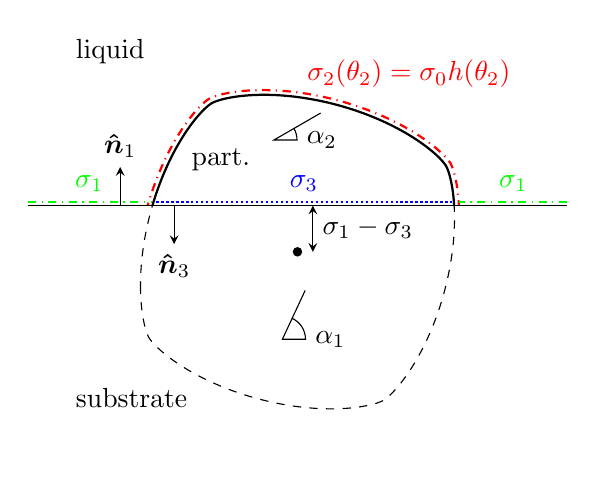
\begin{tikzpicture}[scale=1,font=\normalsize]
	\def\figxwidth{3.5}
	\begin{axis}[
		axis equal,
		disabledatascaling,
		axis line style={draw=none},
		xtick=\empty,
		ytick=\empty,
		xmin=-\figxwidth,xmax=\figxwidth,
		declare function={
			% yshift1=0;
			yshift1=-0.6;
			n=4;
			nsoa=0.9;
			rot1 = 30;
			RW = 0.7*3;
			d=nsoa/(n^2-1);
			aniso1(\t)=1+d*cos(n*(\t-rot1));
			daniso1(\t)=-n*d*sin(n*(\t-rot1));
			Wulffx1(\t) = RW*( aniso1(\t)*cos(\t) - daniso1(\t)*sin(\t) );
			Wulffy1(\t) = RW*( aniso1(\t)*sin(\t) + daniso1(\t)*cos(\t) );
		},
		]
		\begin{scope}
			\clip (axis cs: -\figxwidth,5) rectangle (axis cs:\figxwidth,0);
			\addplot[domain=-pi:pi, samples=150, smooth, thick] ({Wulffx1(deg(x))},{Wulffy1(deg(x))+yshift1});
			\addplot[domain=-pi:pi, samples=150, smooth, red, dash dot, thick] ({1.03*Wulffx1(deg(x))},{1.03*Wulffy1(deg(x))+yshift1});
		\end{scope}
		
		\begin{scope}
			\clip (axis cs: -\figxwidth,-5) rectangle (axis cs:\figxwidth,0);
			\addplot[domain=-pi:pi, samples=150, smooth,dashed] ({Wulffx1(deg(x))},{Wulffy1(deg(x))+yshift1});
		\end{scope}
		
		\path coordinate (C1) at (axis cs:0,yshift1);
		\path coordinate (B1) at (axis cs:-\figxwidth,0);
		\path coordinate (B2) at (axis cs:\figxwidth,0);
		\path coordinate (zz) at  (axis cs:0,0);
		
		% interface specifications
		\draw (B1) -- (B2);
		\draw[green, dash dot, thick] (axis cs:-\figxwidth,0.05) -- node[midway, above] {$\sigma_{1}$} (axis cs:-1.9,0.05);
		\draw[red] (axis cs:0,1.4) node[above right] {$\sigma_{2}(\theta_{2})=\sigma_0 h(\theta_2)$} ;
		\draw[green, dash dot, thick] (axis cs:\figxwidth,0.05) -- node[midway, above] {$\sigma_{1}$} (axis cs:2.1,0.05);
		\draw[blue, densely dotted, thick] (axis cs:-1.83,0.05) -- node [midway, above] {$\sigma_{3}$} (axis cs:2.0,0.05);
		
		\draw[-stealth] (axis cs:-2.3,0) -- (axis cs:-2.3,0.5) node [above] {$\bm{\hat{n}}_1$};
		\draw[-stealth] (axis cs:-1.6,0) -- (axis cs:-1.6,-0.5) node [below] {$\bm{\hat{n}}_3$};
		
		
		\draw[stealth-stealth] (axis cs:0.2,0) -- (axis cs:0.2,yshift1/2) node [right] {$\sigma_1-\sigma_3$} -- (axis cs:0.2,yshift1);
		
		
		\draw[fill] (C1) circle (1.5pt);

		\draw (0.3,1.2) -- ++(-150:0.7) -- ++(0:0.3) node [right] {$\alpha_2$} arc (0:30:0.3) ;
		\draw (0.1,-1.1) -- ++(65-180:0.7) -- ++(0:0.3) node [right] {$\alpha_1$} arc (0:65:0.3) ;
		
		\draw (-3,2) node [right] {liquid};
		\draw (-3,-2.5) node [right] {substrate};
		\draw (-1.5,0.6) node [right] {part.};
	\end{axis}
\end{tikzpicture}

% ISOTROPIC WETTING
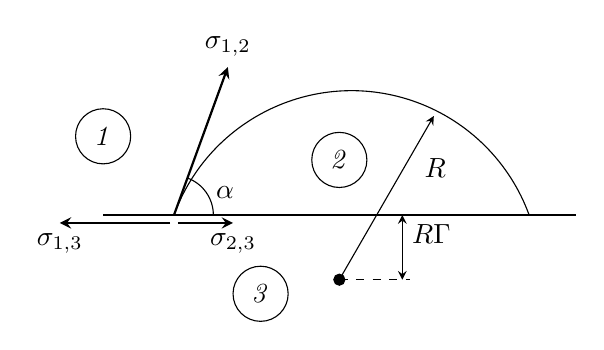
\begin{tikzpicture}[scale=1]
    \newcommand{\ls}{thick};
    \newcommand{\hw}{3};
    \draw[] (-\hw,0) -- (\hw,0);
    \newcommand{\ad}{20};
    \newcommand{\radius}{0.8*\hw};
    \path coordinate (A) at (-0.7*\hw,0);
    \draw (A) arc ((180-\ad):\ad:\radius);
    \path coordinate (C) at (0,-0.821);
    \draw[fill=black] (C) circle (2pt);
    \draw[-stealth] (C) -- ++(60:0.8*\radius) node [below right] {$R$} -- ++(60:0.2*\radius);
     
    \draw[stealth-stealth] (0.8,-0.821) -- (0.8,0) node [below right] {$R\Gamma$};
    % \draw[stealth-stealth] (0.8,-0.821) -- (0.8,0) node [below right] {$R\frac{\sigma_{1,3}-\sigma_{2,3}}{\sigma_{1,2}}$};
    \draw[dashed] (C) -- (0.9,-0.821);
    
    \newcommand{\circs}{0.7cm}
    \draw (-1,-1) node[inner sep=0,circle,draw,minimum size=\circs] {$\mathit{3}$};
    \draw (0,0.7) node[inner sep=0,circle,draw,minimum size=\circs] {$\mathit{2}$};
    \draw (-\hw,1) node[inner sep=0,circle,draw,minimum size=\circs] {$\mathit{1}$};
    
    \newcommand{\la}{2};
    \draw[-stealth,\ls] (A) -- ++(90-\ad:\la) node [above] {$\sigma_{1,2}$};
    \newcommand{\lap}{0.7}  ;
    \draw[-stealth,\ls] (A)++(-0.05,-0.1) -- +(180:2*\lap) node [below] {$\sigma_{1,3}$};
    \draw[-stealth,\ls] (A)++(0.05,-0.1) -- +(0:\lap) node [below] {$\sigma_{2,3}$} ;
    \draw (A)+(0.5,0) arc (0:(90-\ad)/2:0.5) node [right] {$\alpha$} arc ((90-\ad)/2:(90-\ad):0.5);
\end{tikzpicture}

% nucleation_barrier_2D
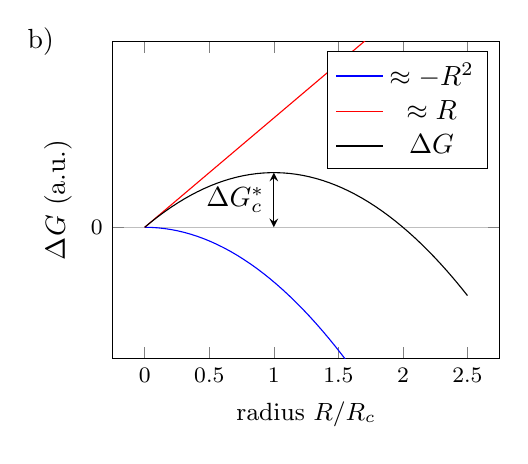
\begin{tikzpicture}
    \newcommand{\sig}{1}
    \newcommand{\dGv}{\sig}
    \newcommand{\barr}{0.5*\sig^2/\dGv}
    \newcommand{\xlim}{2.5}
    \begin{axis}[
        small,
        clip mode=individual,
        xlabel={radius $R/R_c$},
        ytick={0},
        ylabel={$\Delta G$ (a.u.)},
        ylabel near ticks,
        ymin=-1.2,
        ymax=1.7,
        legend entries={$\approx- R^2$,$\approx R$,$\Delta G$},
        legend pos = north east,
        ymajorgrids = true
        ]
        
        \addplot[blue,domain=0:\xlim,samples=50] {-\dGv*x^2/2};
        \addplot[red,domain=0:\xlim,samples=50] {\sig*x};
        \addplot[black,domain=0:\xlim,samples=50] {-\dGv*x^2/2+\sig*x};
        
        \draw[stealth-stealth] (axis cs:1,0) -- (axis cs:1,\barr/2)  node [left] {$\Delta G_c^*$} -- (axis cs:1,\barr);
        
        \draw (rel axis cs: -0.15,1) node [left,inner sep=0] {b)};
    \end{axis}
\end{tikzpicture}

%nucleation_barrier_3D
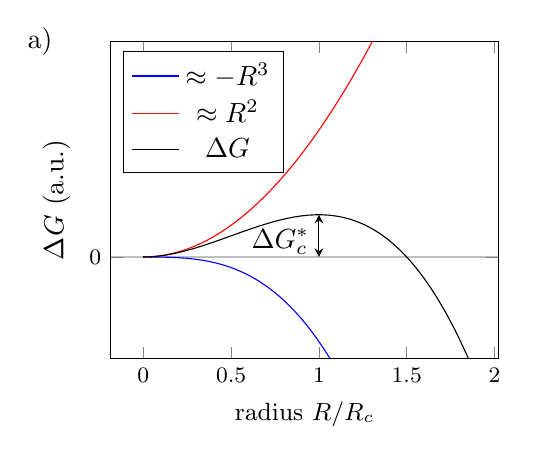
\begin{tikzpicture}
    \newcommand{\sig}{1}
    \newcommand{\dGv}{2*\sig}
    \newcommand{\barr}{2/3*\sig^3/\dGv^2}
    \newcommand{\xlim}{2}
    \begin{axis}[
        small,
        %clip  = false,
        clip mode=individual,
        xlabel={radius $R/R_c$},
        ytick={0},
        ylabel={$\Delta G$ (a.u.)},
        ylabel near ticks,
        ymin=-0.8,
        ymax=1.7,
        legend entries={$\approx- R^3$,$\approx R^2$,$\Delta G$},
        legend pos = north west,
        ymajorgrids = true
        ]
        
        \addplot[blue,domain=0:\xlim,samples=50] {-\dGv*x^3/3};
        \addplot[red,domain=0:\xlim,samples=50] {\sig*x^2};
        \addplot[black,domain=0:\xlim,samples=50] {-\dGv*x^3/3+\sig*x^2};
        
        % \draw[stealth-stealth] (axis cs:1,0) -- (axis cs:1,\barr)  node [above right] {$\Delta G_c^*$};
        \draw[stealth-stealth] (axis cs:1,0) -- (axis cs:1,\barr/2.8)  node [left] {$\Delta G_c^*$} -- (axis cs:1,\barr);
        
        \draw (rel axis cs: -0.15,1) node [left,inner sep=0] {a)};
        %\draw (rel axis cs: -0.15,0) -- (rel axis cs: -0.15,1);
    \end{axis}
\end{tikzpicture}

% wulff_on_GB
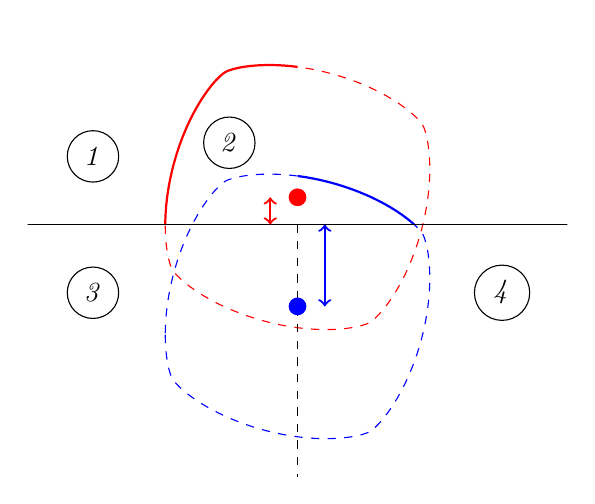
\begin{tikzpicture}
    \begin{axis}[
            axis equal,
            axis line style={draw=none},
            xtick=\empty,
            ytick=\empty,
            declare function={
                yshift1=0.2;
                yshift2=-0.6;
                n=4;
                nsoa=0.9;
                rot1 = 30;
                rot2 = rot1;
                d=nsoa/(n^2-1);
                aniso1(\t)=1+d*cos(n*(\t-rot1));
                daniso1(\t)=-n*d*sin(n*(\t-rot1));
                Wulffx1(\t) = aniso1(\t)*cos(\t) - daniso1(\t)*sin(\t);
                Wulffy1(\t) = aniso1(\t)*sin(\t) + daniso1(\t)*cos(\t);
                aniso2(\t)=1+d*cos(n*(\t-rot2));
                daniso2(\t)=-n*d*sin(n*(\t-rot2));
                Wulffx2(\t) = aniso2(\t)*cos(\t) - daniso2(\t)*sin(\t);
                Wulffy2(\t) = aniso2(\t)*sin(\t) + daniso2(\t)*cos(\t);
                },
        ]
            \begin{scope}
                \clip (axis cs: -2,5) rectangle (axis cs:0,0);
                \addplot[domain=-pi:pi, samples=150, smooth, thick,red] ({Wulffx1(deg(x))},{Wulffy1(deg(x))+yshift1});
            \end{scope}
            
            \begin{scope}
                % \clip (axis cs: -2,-5) rectangle (axis cs:0,0);
                \clip (axis cs: 0,0) -- (axis cs: 0,2) -- (axis cs: 2,2) -- (axis cs: 2,-2) -- (axis cs: -2,-2) -- (axis cs: -2,0) -- cycle (axis cs: 0,0) ;
                \addplot[domain=-pi:pi, samples=150, smooth,red,dashed] ({Wulffx1(deg(x))},{Wulffy1(deg(x))+yshift1});
            \end{scope}
            
            \begin{scope}
                \clip (axis cs: 0,5) rectangle (axis cs:2,0);
                \addplot[domain=-pi:pi, samples=150, smooth,thick,blue] ({Wulffx2(deg(x))},{Wulffy2(deg(x))+yshift2});    
            \end{scope}
            
            \begin{scope}
                % \clip (axis cs: 0,-5) rectangle (axis cs:2,0);
                \clip (axis cs: 0,0) -- (axis cs: 2,0) -- (axis cs: 2,-2) -- (axis cs: -2,-2) -- (axis cs: -2,2) -- (axis cs: 0,2) -- cycle (axis cs: 0,0) ;
                \addplot[domain=-pi:pi, samples=150, smooth,blue,dashed] ({Wulffx2(deg(x))},{Wulffy2(deg(x))+yshift2});    
            \end{scope}
            
            \path coordinate (C1) at (axis cs:0,yshift1);
            \path coordinate (C2) at (axis cs:0,yshift2);
            \path coordinate (B1) at (axis cs:-2,0);
            \path coordinate (B2) at (axis cs:2,0);
            \path coordinate (B3) at  (axis cs:0,-2);
            \path coordinate (zz) at  (axis cs:0,0);
            % \draw[red] (B1) -- (zz);
            % \draw[blue] (B2) -- (zz);
            \draw (B1) -- (B2);
            \draw[dashed] (zz) -- (B3);
            \draw[<->,thick,red] (axis cs:-0.2,0) -- (axis cs:-0.2,yshift1);
            \draw[<->,thick,blue] (axis cs:0.2,0) -- (axis cs:0.2,yshift2);
            
            \draw[fill,red] (C1) circle (3pt);
            \draw[fill,blue] (C2) circle (3pt);
            
            \draw (axis cs:-1.5,0.5) node [circle,draw,minimum size=6] {$\mathit{1}$};
            \draw (axis cs:-0.5,0.6) node [circle,draw,minimum size=6] {$\mathit{2}$};
            \draw (axis cs:-1.5,-0.5) node [circle,draw,minimum size=6]  {$\mathit{3}$};
            \draw (axis cs:1.5,-0.5) node [circle,draw,minimum size=6] {$\mathit{4}$};
            
            % \def\dh{0.1};
            % \def\dw{0.05};
            % \foreach \i in {1,2,...20}{
            %     \draw (\i*\dw,0) -- ((i+1)*\dw,-\dh);
            %     }
            
        \end{axis}
\end{tikzpicture}

% CIRCLE_on_GB
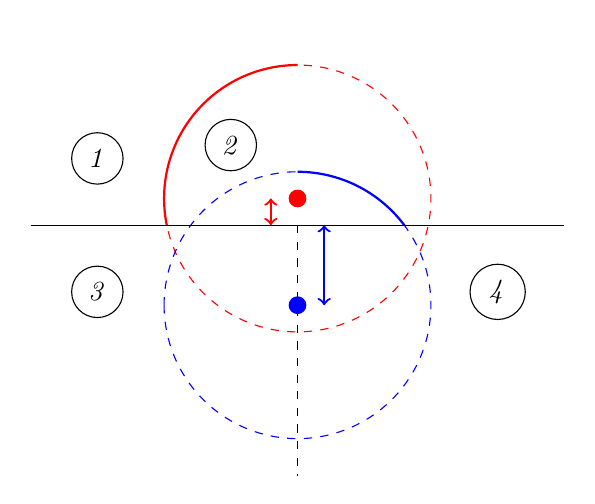
\begin{tikzpicture}
	\begin{axis}[
		axis equal,
		axis line style={draw=none},
		xtick=\empty,
		ytick=\empty,
		declare function={
			yshift1=0.2;
			yshift2=-0.6;
			n=4;
			nsoa=0;
			rot1 = 30;
			rot2 = rot1;
			d=nsoa/(n^2-1);
			aniso1(\t)=1+d*cos(n*(\t-rot1));
			daniso1(\t)=-n*d*sin(n*(\t-rot1));
			Wulffx1(\t) = aniso1(\t)*cos(\t) - daniso1(\t)*sin(\t);
			Wulffy1(\t) = aniso1(\t)*sin(\t) + daniso1(\t)*cos(\t);
			aniso2(\t)=1+d*cos(n*(\t-rot2));
			daniso2(\t)=-n*d*sin(n*(\t-rot2));
			Wulffx2(\t) = aniso2(\t)*cos(\t) - daniso2(\t)*sin(\t);
			Wulffy2(\t) = aniso2(\t)*sin(\t) + daniso2(\t)*cos(\t);
		},
		]
		\begin{scope}
			\clip (axis cs: -2,5) rectangle (axis cs:0,0);
			\addplot[domain=-pi:pi, samples=150, smooth, thick,red] ({Wulffx1(deg(x))},{Wulffy1(deg(x))+yshift1});
		\end{scope}
		
		\begin{scope}
			% \clip (axis cs: -2,-5) rectangle (axis cs:0,0);
			\clip (axis cs: 0,0) -- (axis cs: 0,2) -- (axis cs: 2,2) -- (axis cs: 2,-2) -- (axis cs: -2,-2) -- (axis cs: -2,0) -- cycle (axis cs: 0,0) ;
			\addplot[domain=-pi:pi, samples=150, smooth,red,dashed] ({Wulffx1(deg(x))},{Wulffy1(deg(x))+yshift1});
		\end{scope}
		
		\begin{scope}
			\clip (axis cs: 0,5) rectangle (axis cs:2,0);
			\addplot[domain=-pi:pi, samples=150, smooth,thick,blue] ({Wulffx2(deg(x))},{Wulffy2(deg(x))+yshift2});    
		\end{scope}
		
		\begin{scope}
			% \clip (axis cs: 0,-5) rectangle (axis cs:2,0);
			\clip (axis cs: 0,0) -- (axis cs: 2,0) -- (axis cs: 2,-2) -- (axis cs: -2,-2) -- (axis cs: -2,2) -- (axis cs: 0,2) -- cycle (axis cs: 0,0) ;
			\addplot[domain=-pi:pi, samples=150, smooth,blue,dashed] ({Wulffx2(deg(x))},{Wulffy2(deg(x))+yshift2});    
		\end{scope}
		
		\path coordinate (C1) at (axis cs:0,yshift1);
		\path coordinate (C2) at (axis cs:0,yshift2);
		\path coordinate (B1) at (axis cs:-2,0);
		\path coordinate (B2) at (axis cs:2,0);
		\path coordinate (B3) at  (axis cs:0,-2);
		\path coordinate (zz) at  (axis cs:0,0);
		% \draw[red] (B1) -- (zz);
		% \draw[blue] (B2) -- (zz);
		\draw (B1) -- (B2);
		\draw[dashed] (zz) -- (B3);
		\draw[<->,thick,red] (axis cs:-0.2,0) -- (axis cs:-0.2,yshift1);
		\draw[<->,thick,blue] (axis cs:0.2,0) -- (axis cs:0.2,yshift2);
		
		\draw[fill,red] (C1) circle (3pt);
		\draw[fill,blue] (C2) circle (3pt);
		
		\draw (axis cs:-1.5,0.5) node [circle,draw,minimum size=6] {$\mathit{1}$};
		\draw (axis cs:-0.5,0.6) node [circle,draw,minimum size=6] {$\mathit{2}$};
		\draw (axis cs:-1.5,-0.5) node [circle,draw,minimum size=6]  {$\mathit{3}$};
		\draw (axis cs:1.5,-0.5) node [circle,draw,minimum size=6] {$\mathit{4}$};
		
		% \def\dh{0.1};
		% \def\dw{0.05};
		% \foreach \i in {1,2,...20}{
			%     \draw (\i*\dw,0) -- ((i+1)*\dw,-\dh);
			%     }
		
	\end{axis}
\end{tikzpicture}

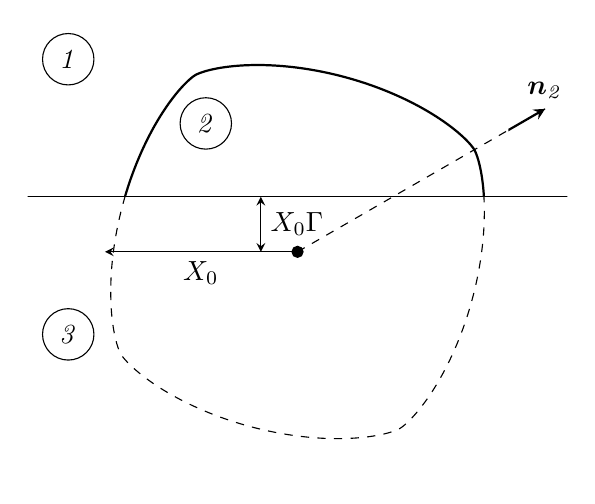
\begin{tikzpicture}
	\begin{axis}[
		axis equal,
		axis line style={draw=none},
		xtick=\empty,
		ytick=\empty,
		declare function={
			% yshift1=0;
			yshift1=-0.6;
			n=4;
			nsoa=0.9;
			rot1 = 30;
			RW = 0.7*3;
			d=nsoa/(n^2-1);
			aniso1(\t)=1+d*cos(n*(\t-rot1));
			daniso1(\t)=-n*d*sin(n*(\t-rot1));
			Wulffx1(\t) = RW*( aniso1(\t)*cos(\t) - daniso1(\t)*sin(\t) );
			Wulffy1(\t) = RW*( aniso1(\t)*sin(\t) + daniso1(\t)*cos(\t) );
		},
		]
		\begin{scope}
			\clip (axis cs: -3,5) rectangle (axis cs:3,0);
			\addplot[domain=-pi:pi, samples=150, smooth, thick] ({Wulffx1(deg(x))},{Wulffy1(deg(x))+yshift1});
		\end{scope}
		
		\begin{scope}
			\clip (axis cs: -3,-5) rectangle (axis cs:3,0);
			\addplot[domain=-pi:pi, samples=150, smooth,dashed] ({Wulffx1(deg(x))},{Wulffy1(deg(x))+yshift1});
		\end{scope}
		
		
		\path coordinate (C1) at (axis cs:0,yshift1);
		\path coordinate (B1) at (axis cs:-3,0);
		\path coordinate (B2) at (axis cs:3,0);
		\path coordinate (zz) at  (axis cs:0,0);
		
		\draw (B1) -- (B2);
		\draw[stealth-stealth] (axis cs:-0.4,0) -- (axis cs:-0.4,yshift1/2) node [right] {$X_0 \Gamma$} -- (axis cs:-0.4,yshift1);
		
		\draw[fill] (C1) circle (2pt);
		\draw[-stealth] (C1) -- (axis cs:-1.055,yshift1) node [below] {$X_0$} -- (axis cs:-2.1,yshift1);
		
		\draw[dashed] (C1) -- (axis cs:2.7,1.5588+yshift1);
		\begin{scope}
			\clip (axis cs: 2.3,0) rectangle (axis cs:3,3);
			\draw[-stealth,thick] (C1) -- (axis cs:2.7,1.5588+yshift1)  node [above] {$\bm{n}_\mathit{2}$};
		\end{scope}
		
		
		
		\draw (axis cs:-2.5,1.5) node [circle,draw,minimum size=6] {$\mathit{1}$};
		\draw (axis cs:-1,0.8) node [circle,draw,minimum size=6] {$\mathit{2}$};
		\draw (axis cs:-2.5,-1.5) node [circle,draw,minimum size=6]  {$\mathit{3}$};
		
	\end{axis}
\end{tikzpicture}

\end{document}
